% -*- mode: latex; coding: latin-1-unix -*- %

\documentclass[12pt]{beamer}
\usepackage[latin1]{inputenc}
\usepackage{multimedia}
\usepackage{pgf}
\usepackage{xcolor}
\usepackage{verbatim}
\usetheme{Darmstadt}
%\usetheme{PaloAlto}

\definecolor{silver}{RGB}{100,150,50}
%\setbeamercolor{structure}{fg=green!65!black}
\setbeamertemplate{background canvas}[vertical shading]%
%[top=silver,bottom=white]
%\textcolor{silver}{quelle jolie couleur}

\AtBeginSection[]
{
  \begin{frame}<beamer>
    \frametitle{Plan}
    \tableofcontents[currentsection, hideothersubsections]
  \end{frame}
}

\logo{
\includegraphics[height=1.0cm]{bx1logo}}

\title{Algorithmes du Monde R�el}
\author
{
    Herv� Descombe\\
    Nicolas Desenne\\
    Xavier Sellier
}
\institute{Universit� de Bordeaux 1 - UFR Informatique}
\date{Master 2 - G�nie logiciel - Semestre 1 - 2008/2009}

\begin{document}

\begin{frame}
  \titlepage
\end{frame}

\begin{frame}
  \frametitle{Plan}
  \tableofcontents %[pausesections]
\end{frame}


\section{R�ductions}
%
% -*- mode: latex; coding: latin-1-unix -*- %


\subsection{Circuit Hamiltonien}

\begin{frame}
\frametitle{Circuit Hamiltonien}
\begin{block}{Rappel du probl\`eme}
  \begin{itemize}
  \item Un graphe G,
  \item Est-ce qu'il existe un circuit qui passe une seule fois par
    tous les sommets de G ?
  \end{itemize}
\end{block}
\end{frame}

\begin{frame}
\frametitle{Circuit Hamiltonien}
\begin{block}{R\'eduction vers SAT}
  \begin{itemize}
  \item Un graphe non orient\'e G
  \item Soit \textit{$x_{ij}$} la variable bool\'eenne qui est \`a
    vraie si le sommet \textit{i} se trouve \`a la j-i\`eme position
  \item Soit \textit{n} le nombre de sommets de G : \textit{n*n}
    variables bool\'eennes.
  \end{itemize}
\end{block}
\end{frame}

\begin{frame}
\frametitle{Circuit Hamiltonien}
\begin{block}{Cinq r\`egles de r\'eduction}
  \begin{itemize}
  \item 1) $\forall j \in V(G), (x_{1j} \vee x_{2j} \vee \ldots \vee
    x_{nj})$
  \item 2) $\forall i$ avec $1 <= i <= n$, $(x_{i1} \vee x_{i2} \vee
    \ldots \vee x_{in})$
  \item 3) $\forall i, 1 <= i <= n, \forall {j, k} \in V(G)$, $j \ne
    k$, $(\neg x_{ij} \vee \neg x_{ik})$
  \item 4) $\forall i, 1 <= i <= n, \forall {j, k} \in V(G), {j,k}
    \notin E(G)$, $(\neg x_{ij} \vee \neg x_{i+1,k})$
  \item 5) $\forall j,k \in V(G)$, ${j,k} \notin E(G)$, $(\neg x_{1j}
    \vee \neg x_{nk})$
  \end{itemize}
\end{block}
\end{frame}

\begin{frame}
\frametitle{Circuit Hamiltonien}
\begin{block}{Variables bool\'eennes}
  \begin{itemize}
  \item Sommet 1 : variables situ\'ees dans [ 1 ; n]
  \item ...
  \item Sommet k : variables situ\'ees dans [ (k+1)*n+1 ; k*n ]
  \end{itemize}
\end{block}
\end{frame}

\subsection{Exemples}

\begin{frame}
\frametitle{Exemples}
\begin{block}{Instance positive}
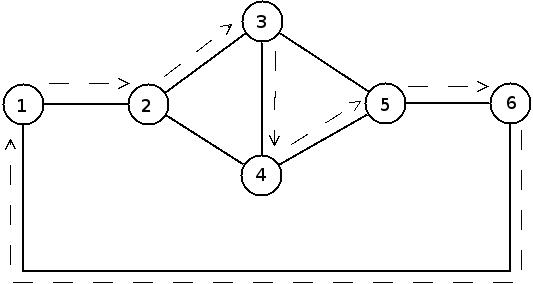
\includegraphics[scale=0.3]{positif.jpeg}
\end{block}
\begin{block}{R\'eponses possibles de SAT}
  \begin{itemize}
  \item R\'eponse : 1 8 15 22 29 36
    \begin{itemize}
    \item (1 2 3 4 5 6)
    \end{itemize}
  \end{itemize}
 \begin{itemize}
  \item R\'eponse : 3 8 13 24 29 34
    \begin{itemize}
    \item (3 2 1 6 5 4)
    \end{itemize}
  \end{itemize}
\end{block}
\end{frame}

\begin{frame}
\frametitle{Exemples}
\begin{block}{Instance n\'egative}
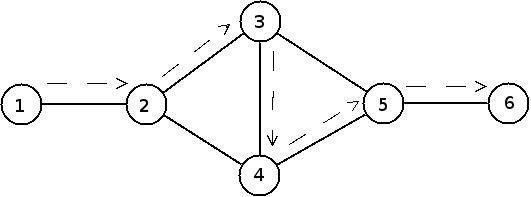
\includegraphics[scale=0.3]{negatif.jpeg}
\end{block}
\begin{block}{R\'eponse de SAT}
  \begin{itemize}
  \item UNSATISFIABLE
  \item Il n'existe pas de circuit hamiltonien pour cete instance.
  \end{itemize}
\end{block}
\end{frame}


\section{Couverture par sommets}
% -*- mode: latex; coding: latin-1-unix -*- %

\begin{frame}[fragile]
\frametitle{Algorithme lin�aire}
\begin{block}{Variables}
\begin{verbatim}

liste feuilles;
liste couverture;
int[] pere;
int[] nbFils;
int racine;

\end{verbatim}
\end{block}


\begin{block}{Initialisation}
\begin{verbatim}
function void algo(){
int i := feuilles.premier();
Si i := racine;
  alors fin algo;
\end{verbatim}
\end{block}

\end{frame}

\begin{frame}[fragile]
\frametitle{Algorithme lin�aire}
\begin{block}{Traitement}
\begin{verbatim}
int j := pere[i];
int k := pere[j];

feuilles.supprimerEnTete();
couverture.ajouterEnTete(j);

pere[j] := 0;
pere[i] := 0;
\end{verbatim}
\end{block}
\end{frame}

\begin{frame}[fragile] 
\begin{block}{Fin}
\begin{verbatim}
Si k != 0
   alors nbFils[k]--;
         Si nbFils[k] = 0
            alors feuilles.ajouterEnTete(k);
algo();
}
\end{verbatim}
\end{block}
\end{frame}

\begin{frame}
\frametitle{Algorithme lin�aire}
\begin{block}{Exemple}
\begin{center}
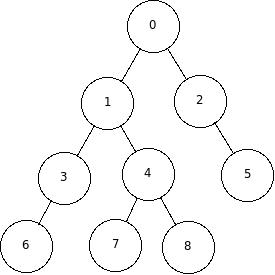
\includegraphics[scale=0.7]{arbre9sommets}
\end{center}
\end{block}
\end{frame}

\begin{frame}
\frametitle{Algorithme lin�aire}
\begin{block}{Exemple}
\begin{center}
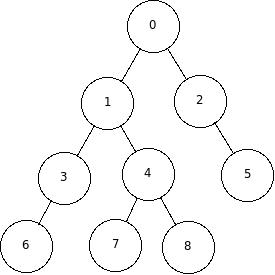
\includegraphics[scale=0.4]{arbre9sommets}\\
couverture : 3
\end{center}
\end{block}
\end{frame}

\begin{frame}
\frametitle{Algorithme lin�aire}
\begin{block}{Exemple}
\begin{center}
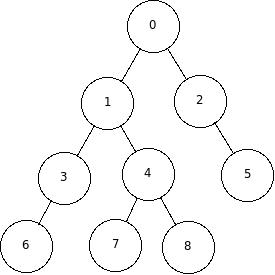
\includegraphics[scale=0.4]{arbre9sommets}\\
couverture : 3 - 4
\end{center}
\end{block}
\end{frame}

\begin{frame}
\frametitle{Algorithme lin�aire}
\begin{block}{Exemple}
\begin{center}
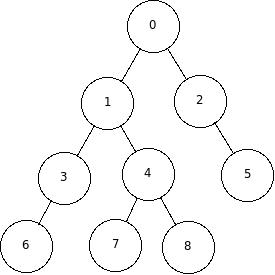
\includegraphics[scale=0.4]{arbre9sommets}\\
couverture : 3 - 4 - 2
\end{center}
\end{block}
\end{frame}

\begin{frame}
\frametitle{Algorithme lin�aire}
\begin{block}{Exemple}
\begin{center}
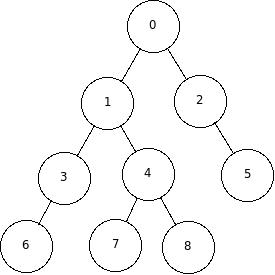
\includegraphics[scale=0.4]{arbre9sommets}\\
couverture : 3 - 4 - 2 - 0
\end{center}
\end{block}
\end{frame}

\begin{frame}[fragile]
\frametitle{Algorithme lin�aire}
\begin{block}{Fichier gengraph}
\begin{verbatim}
0-1 0-2 1-3 1-4 3-6 4-7 4-8 2-5
\end{verbatim}
\end{block}

\begin{block}{R�sultat}
\begin{verbatim}
0 2 3 4
\end{verbatim}
\end{block}
\end{frame}


\section{Algorithmes d'approximation}
% -*- mode: latex; coding: latin-1-unix -*- %

\subsection{Comparaison}

\begin{frame}
\frametitle{Arbre 5 sommets}
\begin{center}
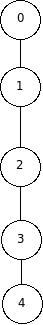
\includegraphics[scale=0.6]{arbre5sommets}
\end{center}
\end{frame}

\begin{frame}
\frametitle{Comparaison entre l'algorithme optimal et l'algorithme 2-approch�}
\begin{block}{Sur un arbre � 5 sommets - Temps d'execution}
  \begin{itemize}
  \item Algorithme optimal : 0,016 secondes
  \item Algorithme 2-approch� : 0,003 secondes
  \end{itemize}
\end{block}
\begin{block}{Sur un arbre � 5 sommets - R�sultats}
  \begin{itemize}
  \item Algorithme optimal : 1 3
  \item Algorithme 2-approch� : 1 3
  \end{itemize}
\end{block}
\end{frame}


\begin{frame}
\frametitle{Arbre 9 sommets}
\begin{center}
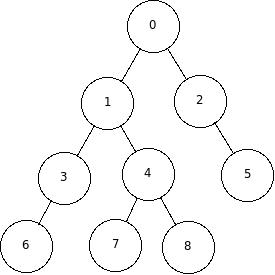
\includegraphics[scale=0.7]{arbre9sommets}
\end{center}
\end{frame}

\begin{frame}
\frametitle{Comparaison entre l'algorithme optimal et l'algorithme 2-approch�}
\begin{block}{Sur un arbre � 9 sommets - Temps d'execution}
  \begin{itemize}
  \item Algorithme optimal : 0,013 secondes
  \item Algorithme 2-approch� : 0,006 secondes
  \end{itemize}
\end{block}
\begin{block}{Sur un arbre � 9 sommets - R�sultats}
  \begin{itemize}
  \item Algorithme optimal : 1 2 3 4
  \item Algorithme 2-approch� : 0 2 3 4
  \end{itemize}
\end{block}
\end{frame}


\begin{frame}
\frametitle{Arbre 15 sommets}
\begin{center}
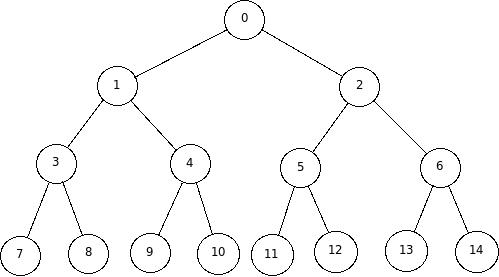
\includegraphics[scale=0.6]{arbre15sommets}
\end{center}
\end{frame}

\begin{frame}
\frametitle{Comparaison entre l'algorithme optimal et l'algorithme 2-approch�}
\begin{block}{Sur un arbre � 15 sommets - Temps d'execution}
  \begin{itemize}
  \item Algorithme optimal : 0,030 secondes
  \item Algorithme 2-approch� : 0,007 secondes
  \end{itemize}
\end{block}
\begin{block}{Sur un arbre � 15 sommets - R�sultats}
  \begin{itemize}
  \item Algorithme optimal : 0 3 4 5 6
  \item Algorithme 2-approch� : 0 3 4 5 6
  \end{itemize}
\end{block}
\end{frame}

\begin{frame}
\frametitle{Graphe 20 sommets}
\begin{center}
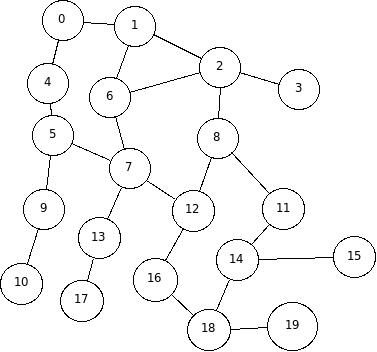
\includegraphics[scale=0.6]{graphe20sommets}
\end{center}
\end{frame}

\begin{frame}
\frametitle{Comparaison entre l'algorithme optimal et l'algorithme 2-approch�}
\begin{block}{Sur un graphe � 20 sommets - Temps d'execution}
  \begin{itemize}
  \item Algorithme optimal : 0,028 secondes
  \item Algorithme 2-approch� : 0,006 secondes
  \end{itemize}
\end{block}
\begin{block}{Sur un graphe � 20 sommets - R�sultats}
  \begin{itemize}
  \item Algorithme optimal : 1 2 4 7 8 9 13 14 16 19 (10 sommets)
  \item Algorithme 2-approch� : 0 1 2 5 7 8 9 11 12 13 14 16 18 (13 sommets)
  \end{itemize}
\end{block}
\end{frame}

\begin{frame}
\frametitle{Comparaison entre l'algorithme optimal et l'algorithme 2-approch�}
\begin{block}{Sur un graphe � 40 sommets - Temps d'execution}
  \begin{itemize}
  \item Algorithme optimal : 0,078 secondes
  \item Algorithme 2-approch� : 0,008 secondes
  \end{itemize}
\end{block}
\begin{block}{Sur un graphe � 40 sommets - R�sultats}
  \begin{itemize}
  \item Algorithme optimal : 34 sommets
  \item Algorithme 2-approch� : 37 sommets
  \end{itemize}
\end{block}
\end{frame}

\begin{frame}
\frametitle{Comparaison entre l'algorithme optimal et l'algorithme 2-approch�}
\begin{block}{Sur un graphe � 100 sommets - Temps d'execution}
  \begin{itemize}
  \item Algorithme optimal : 0,268 secondes
  \item Algorithme 2-approch� : 0,015 secondes
  \end{itemize}
\end{block}
\begin{block}{Sur un graphe � 100 sommets - R�sultats}
  \begin{itemize}
  \item Algorithme optimal : 95 sommets
  \item Algorithme 2-approch� : 99 sommets
  \end{itemize}
\end{block}
\end{frame}


\subsection{Instance Critique}

\begin{frame}
\frametitle{Arbre � n sommets}
\begin{center}
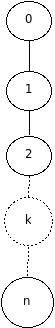
\includegraphics[scale=0.6]{instancecritique}
\end{center}
\end{frame}


\begin{frame}
\frametitle{Sur un arbre de 10 noeuds}
\begin{block}{Un arbre a un seul fils a chaque fois}
  \begin{itemize}
  \item Algorithme optimal : 0,005 secondes - 5 sommets
  \item Algorithme 2-approch� : 0,005 secondes - 10-1 sommets
  \end{itemize}
\end{block}
\end{frame}

\begin{frame}
\frametitle{L'algorithme approch� en instance critique}
\begin{block}{Un arbre a un seul fils a chaque fois}
  \begin{itemize}
  \item L'algorithme approch� va prendre tous les neouds
  \item Le temps de calcul sera faible, mais la quantit� de m�moire
    consomm�e sera doubl�e par rapport � la solution optimale.
  \end{itemize}
\end{block}
\end{frame}



\section{Conclusion}
%% -*- mode: latex; coding: latin-1-unix -*- %
\subsection{Conclusion}

\begin{frame}
\frametitle{Conclusion}
\begin{block}{Bilan du projet XP}
  \begin{itemize}
  \item Projets r�utilisant du code, non adapt�s � XP
  \item Code fourni peu document�
  \end{itemize}
\end{block}
\end{frame}


\end{document}
